\section{Mobile CRM-systems review}\label{sec:review}

As the mobile device has all necessary information of calls, it is desirable for the application to automatically register a call in CRM-system. It is necessary to carry out the analysis of applications of popular systems. Analysis purpose is to reveal the existence of the module of automatic registration of the calls connected to the client base of the company.

To find out the existence of this module for the chosen set of systems the following operations have been performed:

\begin {itemize}
\item The account of the user was created.
\item The contact with the known phone number was added.
\item The application of target CRM was installed on the smartphone with Android OS.
\item A call from the mobile application to the registered contact was made.
\item A call from the registered contact to the smartphone with the installed application was made.
\item The Events/calls tab and the existence of the registered call in it was checked.
\end {itemize}

As a result of the experiment the results presented in table \ref{fig:appReview} have been received

\begin{figure}[tbh]
\centering
\caption{Applications possibility}
\label{fig:appReview}
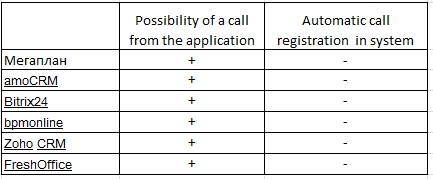
\includegraphics[width=\linewidth]{appReview}
\end{figure}
